\documentclass[sn-mathphys,Numbered]{sn-jnl}

\usepackage{graphicx}
\usepackage{multirow}
\usepackage{amsmath,amssymb,amsfonts}
\usepackage{amsthm}
\usepackage{mathrsfs}
\usepackage[title]{appendix}
\usepackage[table]{xcolor}
\usepackage{textcomp}
\usepackage{manyfoot}
\usepackage{booktabs}
\usepackage{algorithm}
\usepackage{algorithmicx}
\usepackage{algpseudocode}
\usepackage{listings}

\usepackage{microtype}
\usepackage[caption=false]{subfig}
\usepackage{url}
\usepackage[shortlabels]{enumitem}
\usepackage[export]{adjustbox}
\usepackage{bm}
\graphicspath{{fig/}}
\usepackage[utf8]{inputenc} 
\usepackage[T1]{fontenc}    
\usepackage{geometry}

\theoremstyle{thmstyleone}
\newtheorem{theorem}{Theorem}
\newtheorem{proposition}[theorem]{Proposition}
\newtheorem{lemma}[theorem]{Lemma}
\newtheorem{corollary}[theorem]{Corollary}

\theoremstyle{thmstyletwo}
\newtheorem{example}{Example}
\newtheorem{remark}{Remark}

\theoremstyle{thmstylethree}
\newtheorem{definition}{Definition}
\newtheorem{assumption}{Assumption}

\def\cO{\mathcal{O}}
\def\unif{\mathrm{Unif}}
\def\rank{\mathrm{rank}}
\def\supp{\mathrm{supp}}
\def\sign{\mathrm{sign}}
\DeclareMathOperator*{\argmin}{arg\,min}
\DeclareMathOperator*{\minimize}{\mathrm{minimize}}
\DeclareMathOperator*{\subject}{\mathrm{subject~to~}}

\newcommand{\BK}[1]{{\textcolor{cyan}{#1}}}

\raggedbottom

\begin{document}

\title[Inspect]{Bridging The Gap Between Local And Global Derivative-Free Optimization Methods - Inspect as You Run}

\author[1]{\fnm{Bumsu} \sur{Kim}}\email{bumsu@math.ucla.edu}

\author*[2]{\fnm{Wotao} \sur{Yin}}\email{wotao.yin@alibaba-inc.com}
\equalcont{These authors contributed equally to this work.}

\affil[1]{\orgdiv{Department of Mathematics}, \orgname{University of California, Los Angeles}, \orgaddress{ \city{Los Angeles}, \postcode{90095}, \state{CA}, \country{USA}}}

\affil*[2]{\orgdiv{Decision Intelligence Lab, DAMO Academy}, \orgname{Alibaba US}, \orgaddress{\city{Bellevue}, \postcode{98004}, \state{WA}, \country{USA}}}

\abstract{ TBU }

\keywords{Derivative-free optimization, Zeroth-order optimization}

\pacs[MSC Classification]{65K05, 68Q25, 90C56}

\maketitle
\section{Introduction}
Brief introduction to the DFO problems. and explain local methods, model-based global methods and their limitations.

\subsection{The gap between global optimization and local optimization}
The majority of the optimization methods are either global optimization or local optimization methods. They approach these problems in very different ways, which creates a gap between them. 

\paragraph{Global Optimization} This class of methods aims to find the absolute best solution (up to a small tolerance) in the \emph{entire} solution space for an optimization problem. In other words, it searches for the overall minimum or maximum. The techniques used for global optimization are typically exhaustive, as they have to explore the entire problem space to ensure they have found the best possible solution up to the tolerance. This is because there may be many local optima, but only one (or a few) global optima. As a result, these methods can be computationally expensive, particularly for complex, high-dimensional problems.

\paragraph{Local Optimization} This class of methods, on the other hand, focuses on finding a good solution in a neighborhood, no matter how small it is, of a specific point in the solution space. This does not necessarily mean that the solution will be the best overall; instead, it means that there is no better solution in some vicinity of the found one. Thus, local optimization methods can be faster and less computationally expensive than global ones, but they may miss the global optimum if it lies outside of the selected neighborhood.

\paragraph{Gap between these two types of optimization} The gap can be understood through the following perspectives.

Global optimization guarantees the best solution, while local optimization only guarantees the best solution within a local neighborhood. However, the size of the neighborhood is not known or controllable.

Due to the need to explore the entire solution space, global optimization usually requires much more computational effort, causing much longer running time, than local optimization.

In practice, the choice between local and global optimization often depends on the specific problem, the resources available, and the acceptable trade-offs. For low-dimensional problems where it is crucial to find the absolute best solution, global optimization becomes necessary. However, for many problems, a solution that is ``good enough'' is sufficient. 

Local methods, despite only producing local solutions, may be preferred and sometimes are only the choice due to their efficiency. 
To improve the solution quality of local methods, meta-heuristics were introduced. They include using multiple starting points, simulated annealing, genetic algorithms that allow occasional moves in the worse direction, etc.
However, neither local methods nor their meta-heuristic improvements could quantify how ``good enough'' their solutions are.

\paragraph{Filling the gap by $R$-local optimization}
According to \cite{chen2019run}, 
an $R$-local minimizer is a type of local minimizer that specifies a radius of the local neighborhood around the minimizer.

More specifically, suppose we would like to minimize a function $f: \mathbb{R}^n \rightarrow \mathbb{R}$. We say that $x^\star\in\mathbb{R}^n$ is an $R$-local minimizer of $f$ if  that $x^\star$ is a  minimizer of $f$ in the closed ball ${x \in \mathbb{R}^n: \|x - x^\star\| \leq R}$.
This means $x^\star$ is a local minimizer in the neighborhood of radius $R$ around it. 

The concept of an $R$-local minimizer is often used when we want to guarantee the solution found to have a sufficient quality in a vicinity of a defined size. This can be helpful when the global minimizer cannot be easily found or when the function is too complex to optimize over its entire domain. The value of $R$ could be chosen based on some prior knowledge or through a process of trial and error.

\subsection{DFO and $R$-local optimization}
$R$-local optimization offers clear advantages over purely local methods in terms of discovering better solutions. However, it often incurs a higher computational cost, specifically requiring \BK{$\mathcal{O}(s \exp({O(d')}))$ samples for $s$ blocks of dimension $d'$ as shown in \cite{chen2019run}}.
This can become prohibitively expensive in certain scenarios\BK{, particularly when the cost of sampling the objective function and its gradient is approximately equal}. However, in derivative-free optimization, unless there are special structures (such as sparse gradients described in \cite{cai2020zeroth}), an additional factor of $d$, compared to its gradient-based counterpart, in the sample complexity is unavoidable. Consequently, performing inspections may not significantly impact the overall sample complexity, but only up to a constant factor.

\section{Main Results}
Suppose that we have a local DFO method (e.g. Nesterov-Spokoiny\cite{nesterov2017random}, or CARS\cite{kim2021curvature}) that consumes up to $\mathcal{O}(d^\nu)$ queries per iteration. (for instance, $\nu = 0$ for CARS, and $\nu=1$ for AdaDGS. For Nesterov-Spokoiny, $\nu$ is typically 0 or 1, depending on the level of approximation to the Monte-Carlo approximation).
The main idea is to use additional queries, up to the same $\mathcal{O}(d^\nu)$, to drive the method to converge to an $R$-local minima with high probability. The resulting algorithm thus requires the same order of magnitude in terms of function queries.
In addition to that, we want it to be a model-free algorithm, meaning that we don't set up a global surrogate model for the problem, which is often quite expensive when $d$ is large.



\begin{definition}[Successful Inspection] Given a descent threshold $\nu$, an inspection at a point $y$ around $x$ is said to be successful $\nu \geq 0$ if $f(y) < f(x) - \nu$.
\end{definition}


\begin{algorithm}[H]
\caption{Inspect as You Run}
 \label{alg:IR general}
\begin{algorithmic}[1]
  \State \textbf{Input:} $x_0$: initial point; $r$: sampling radius; $R$: inspection radius; $\mathcal{A}$: One step of a DFO method, generating the next iterate; $n_k$: maximum number of inspections at $k$-th iteration; $\nu$: descent threshold
  \State Get the oracle $f(x_0)$.
  \For{$k = 1, \cdots, K$}
        \State Compute $x_{k, 0} = \mathcal{A}(x_k)$
        \For {$j = 1, \cdots, n_k$}
            \State Compute $f(x_{k,j})$ 
            \If{$f(x_{k,j}) < f(x_{k,0}) - \nu$}
                \State Set $x_{k+1} = x_{k,j}$ and \emph{break}
            \EndIf
        \EndFor
        \State If no successful inspections, set $x_{k+1} = x_{k,0}$ \label{eq: inspection step in the algorithm 1}
  \EndFor
   \State \textbf{Output:} $x_K$: estimated optimum point.
\end{algorithmic}
\end{algorithm}

\subsection{Analysis}
% In this section we largely depend on the analysis in \cite{chen2019run} to guarantee the convergence of this plug-in algorithm to an appropriate point.
% First we introduce a blockwise $\mathbf{R}$-local minimizer, which generalizes the $R$-local minimizer.

% Cite Run-and-Inspection paper's results

% When $f$ has a form $g + \rho$, where $g$ has $L$-Lipschitz gradient and is Polyak-{\L}ojasiewicz (PL), and $\rho$ satisfies:
% \begin{align*}
%     |\rho(x)- \rho(y)| \leq \alpha \|x-y\| + 2\beta ,
% \end{align*}
In this section, we provide an analysis for the point obtained from Algorithm~\ref{alg:IR general}.
Roughly speaking, if the recent $M$ inspections did not give a better point than the local DFO method $\mathcal{A}$, it is an $R_0$-local minimum with probability at least $1 - \exp(-\mathcal{O}(M))$, for some $R_0 < R$.

We assume the objective function $f$ satisfies the conditions for the DFO method $\mathcal{A}$ to converge. In addition, we also assume $f$ is $\bar{L}$-Lipschitz continuous. Note that, however, if $\nabla f$ is already assumed to be Lipschitz, like in the analyses of many methods, the assumption implies the Lipschitz continuity of $f$.

% Although a local DFO method that estimates the derivatives by finite difference can smooths out the effect of $\beta$ with large sampling radius $r$, they also blow up if $r$ is too small. Thus we assume $\beta= 0$ here for a simpler analysis.
% In practice, one can use an appropriate lower bound for $r$ to achieve an approximate optimum.
% thus  for instance, $O(\varepsilon^{1/4})$ for CARS 

% Theorem 5 in \cite{chen2019run} gives a sufficient condition for a $\mathbf{R}$-local minimizer $\bar{x}$ being an approximate global minimizer. Furthermore, Theorem 7 states that an \emph{approximate} $\mathbf{R}$-local minimizer can also be one. Finally, Theorem 9 addresses the condition to guarantee an approximate $\mathbf{R}$-local minimizer.



For CARS \cite{kim2021curvature}, for instance, it originally uses 4 (CARS, the vanilla version) or 5 (CARS-CR) queries per iteration. Thus by adding, for instance, 3 queries for inspection per iteration, we have the IR version of CARS, whose cost is up to 75\% more than the original method per iteration.

In particular, for convex problems the overall cost will be increased with at most a constant factor. However, we argue that with inspection one can find significantly better local minima for a certain class of nonconvex problems.

\begin{theorem} \label{thm: high prob guarantee of an approx. R-local min}
    Let $\{x_k\}_{k=1}^{K}$ be the sequence of points obtained from Algorithm~\ref{alg:IR general}. Assume that no successful inspections occur for all $k \geq k_0$, and let $m$ be the total number of inspections for $k \geq k_0$. Suppose
    \begin{align*}
        \|x_{k} - x_K\| \leq D < R \quad \text{for all } k \geq k_0.
    \end{align*}
    Define $R_0 = R-D$ and choose a positive $\tilde{r} < D$. Then, $x_K$ is an $R_0$-local minimum up to $\eta = \bar{L}\tilde{r} + \nu$ with probability at least $1-\exp(- m (\tilde{r}/R)^d)$.
\end{theorem}
\begin{proof}
    Begin by noting that the ball $B(x_K, R_0 + \tilde{r})$ is a subset of $B(x_{k}, R)$ for all $k \geq k_0$. Hence, for a random variable $z \sim \mathrm{Unif}(B(x_{k}, R))$, the conditioned random variable $z|\mathcal{A}$, where $\mathcal{A}$ is the event $z \in B(x_K, R_0 + \tilde{r})$, follows the uniform distribution over $B(x_K, R_0 + \tilde{r})$.

    At iteration $k= K$, define $S = \{y_i\}_{i=1}^{M}$ as the subset of the recent $m$ inspection points contained within $B(x_K, R_0 + \tilde{r})$. Then $M$ follows the binomial distribution $M \sim \mathrm{Binomial}( m , \phi_1)$ with $\phi_1 = \left(\frac{R_0  + \tilde{r}}{R}\right)^d$.
    
    We now demonstrate that if $S$ is sufficiently dense, $x_K$ becomes an approximate $R_0$-local minimum. Consider
    \begin{align*}
        \tilde{x} := \argmin_{x \in B(x_K, R_0)} f(x).
    \end{align*}
    If there exists $y_i \in S \cap B(\tilde{x},\tilde{r})$, knowing $y_i$ is not a successful inspection, we obtain 
    \begin{align*}
        f(x_K) \leq f(\tilde{x}) + (f(y_i) - f(\tilde{x})) + \nu
        \leq \min_{x \in B(x_K, R_0)}f(x) + \bar{L} \tilde{r} + \nu,
    \end{align*}
    implying that $x_K$ is an $R_0$-local minimum up to $\eta = \bar{L}\tilde{r} + \nu$.
    
    Finally, we need to find the probability bound for $S \cap B(\tilde{x}, \tilde{r})$ not being empty. As each $y_j \sim \mathrm{Unif}(B(x_K, R_0 + \tilde{r}))$ and $B(\tilde{x},\tilde{r}) \subseteq B(x_K, R_0 + \tilde{r})$, we get $\phi_2 := \mathbb{P}[y_j \in B(\tilde{x}, \tilde{r})] = \left(\frac{\tilde{r}}{R_0 + \tilde{r}}\right)^d$. Consequently,
    \begin{align*}
        & \quad~\mathbb{P}[y_j \not\in B(\tilde{x}, \tilde{r}) \text{ for all } j = 1, \cdots, M] \\
        & =\sum_{M' = 0}^{\infty} \left(1 - \phi_2\right)^{M'} \mathbb{P}[M = M'] \\
        & =\mathbb{E}_{M}(\exp{(M\log(1-\phi_2))}) \\
        & \stackrel{(a)}{=} (1-\phi_1 + \phi_1 \exp{(\log(1-\phi_2))})^m \\
        & = (1-\phi_1 \phi_2 )^m \\
        & \leq \exp(-m\phi_1 \phi_2), & \text{($1-x \leq \exp(-x)$)}
    \end{align*}
    where (a) is from the moment generating function formula for binomial distributions.
    And since $\phi_1 \phi_2 = (\tilde{r}/R)^d$, $S \cap B(\tilde{x}, \tilde{r})$ is nonempty with a probability of at least $1 - \exp(-m (\tilde{r}/R)^d)$.
\end{proof}



Theorem~\ref{thm: high prob guarantee of an approx. R-local min} states that when we are near the local minimum found by a DFO method, we can guarantee, with probability $1-\delta$, it is indeed an approximate $R_0$-local minimum with a total number of $\log(\delta^{-1}) \left(\frac{R}{\tilde{r}}\right)^d$ inspections.

% Description/Explanation on the Algorithm and its analysis
% $\tilde{r} > 0$, which is used to describe the \emph{density} of the sampled points in \cite{chen2019run}. Then consider 
% For a local DFO method $\mathcal{A}$, we say an iterate $x_k$ satisfies $\mathcal{Q}_1(\mathcal{A}, D)$\BK{proper name of it?} if
% $\|x_{k+i} - x_{k+j}\| \leq D$ for all $i, j \geq 0$.
% Note that when $x_k$ satisfies $\mathcal{Q}(\mathcal{A}, D)$ with $D < R$, then for any $R_0 \leq R - D$, $B(x_K, R_0) \subseteq B(x_{K'}, R)$ for all $K, K' \geq k$. Thus if $z \sim \mathrm{Unif}(B(x_{K'}, R)$, the conditioned random variable $y' := y | [y \in B(x_K, R_0)]$ is uniformly distributed on $B(x_K, R_0)$. Also note that the probability of $y \in B(x_K, R_0)$ is $\left({R_0}/{R}\right)^d =: \phi_1$.




\section{Experimental Results}
\subsection{Spurious Local Minima}
Quadratic Plus Sine function 
\begin{figure*}
    \centering
    \raisebox{-0.5\height}{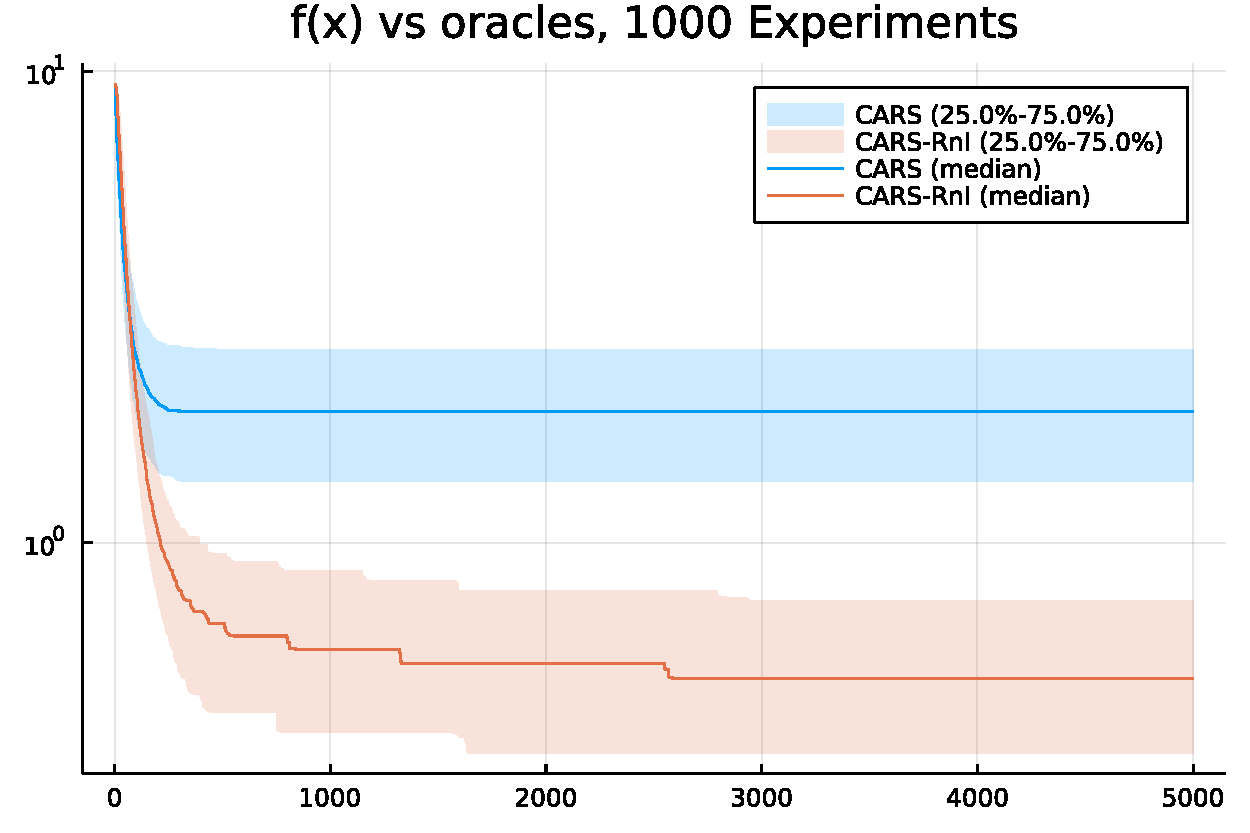
\includegraphics[width=0.48\linewidth]{fig/freq10_amp0.2_quad_plus_sin.pdf}}
    \raisebox{-0.5\height}{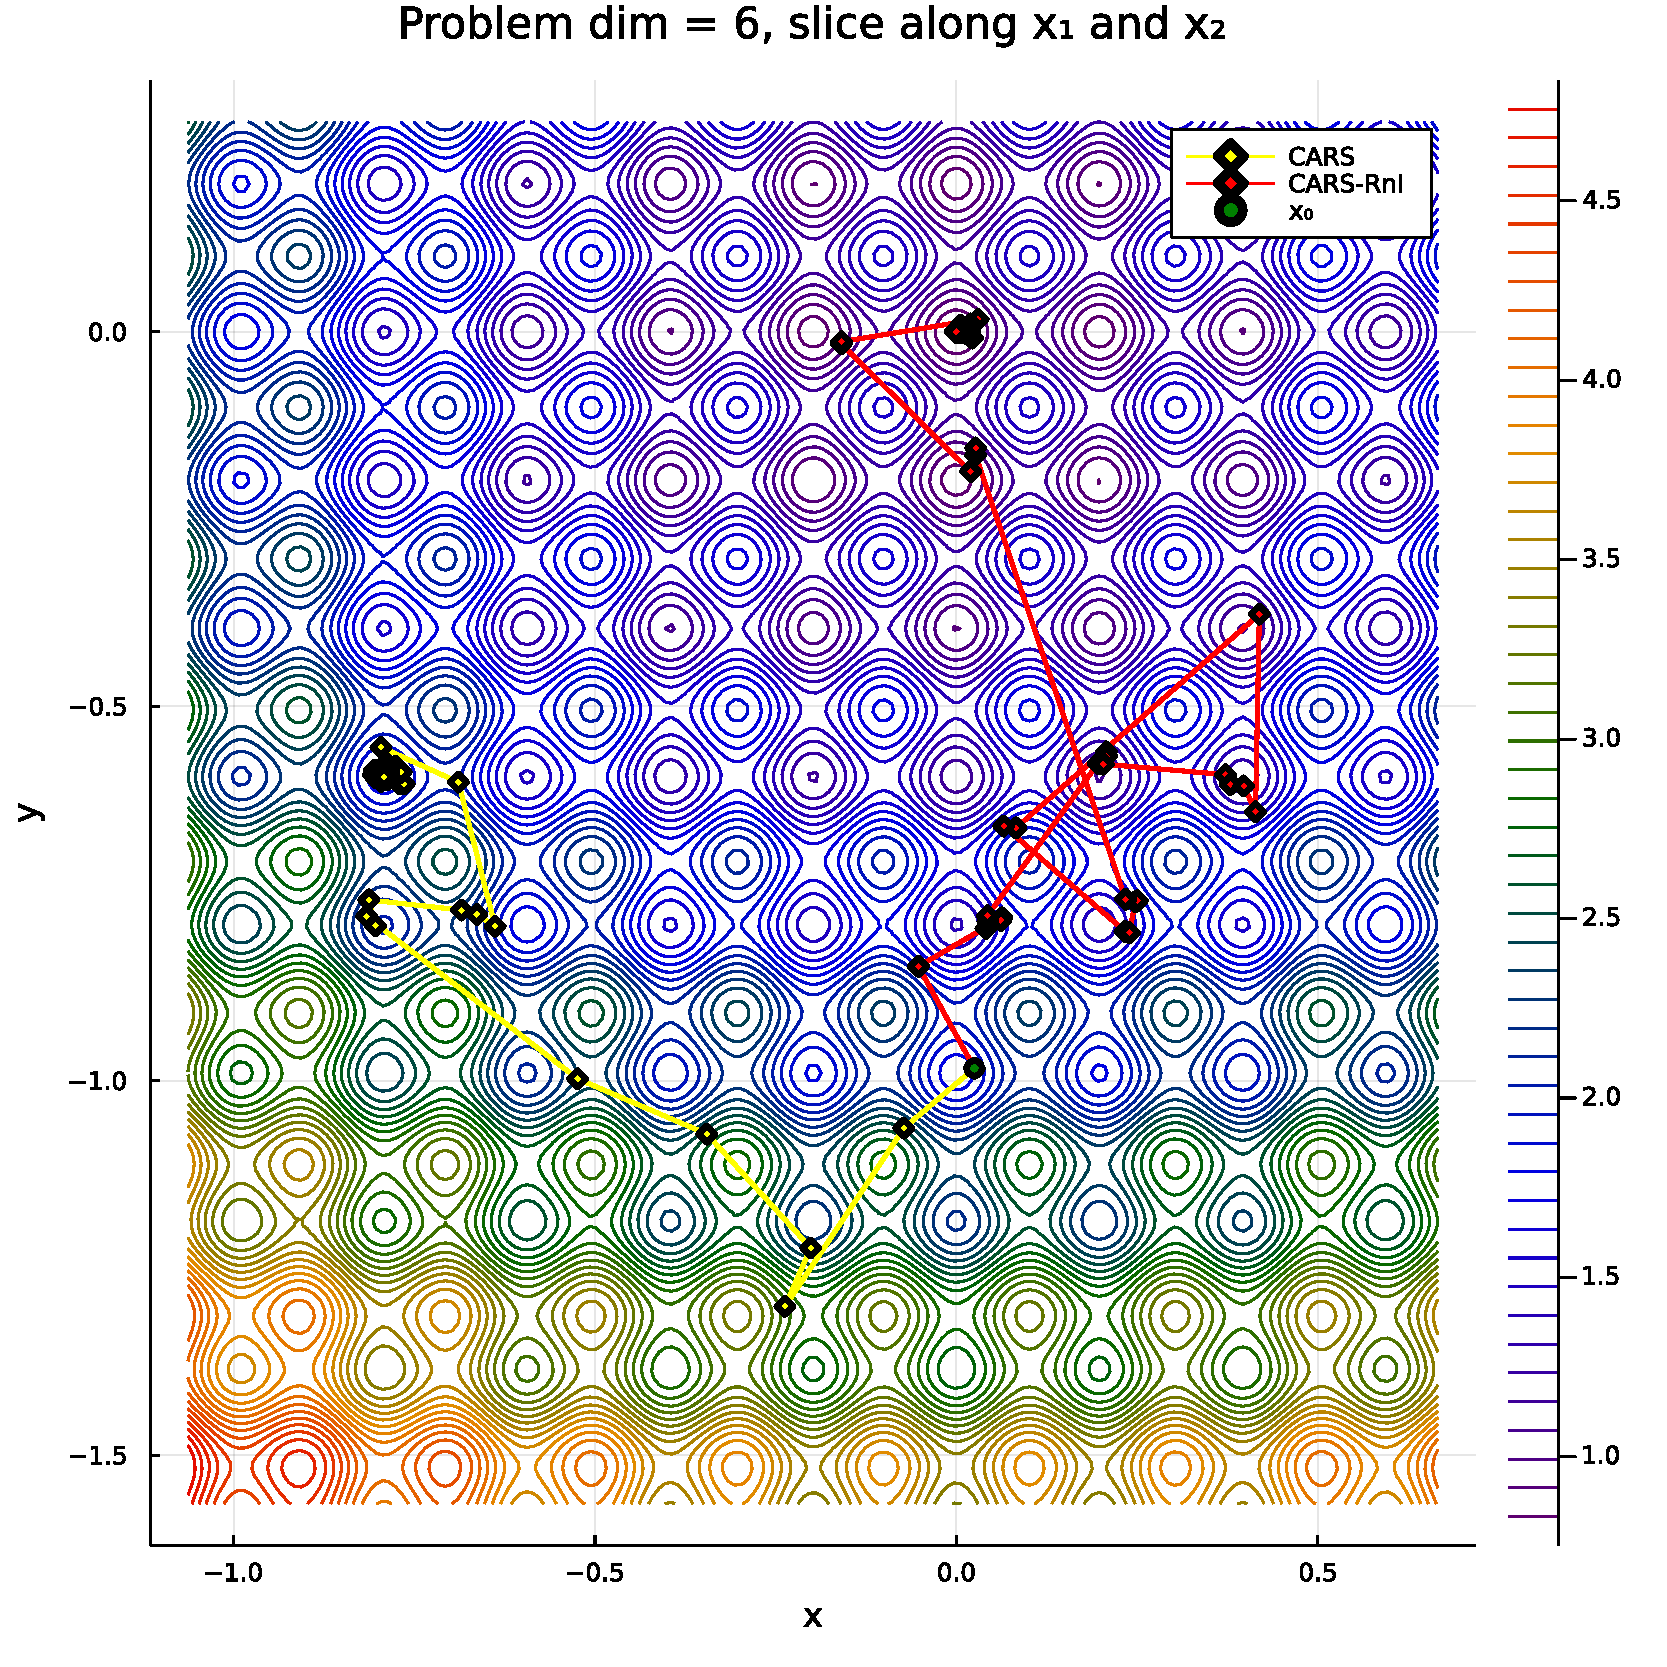
\includegraphics[width=0.48\linewidth]{fig/freq10_amp0.2_quad_plus_sin_sols.pdf}}
    \caption{Comparison of CARS and the Inspect-as-Running version of CARS for the quad+sine function}
    \label{fig:Convex plus sine}
\end{figure*}

\subsection{Ackley's Functions}
Example from \cite{chen2019run}
\begin{figure*}
    \centering
    \raisebox{-0.5\height}{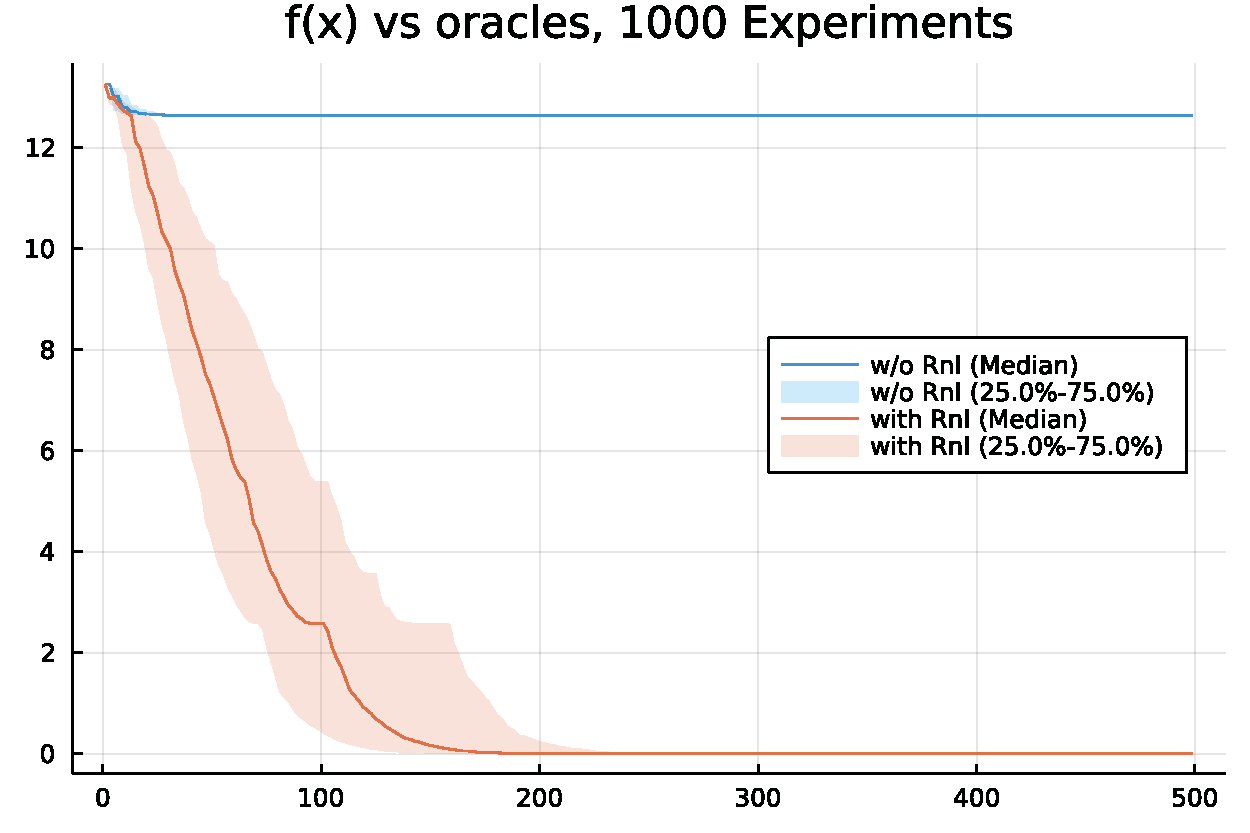
\includegraphics[width=0.48\linewidth]{fig/Ackley.pdf}}
    \raisebox{-0.5\height}{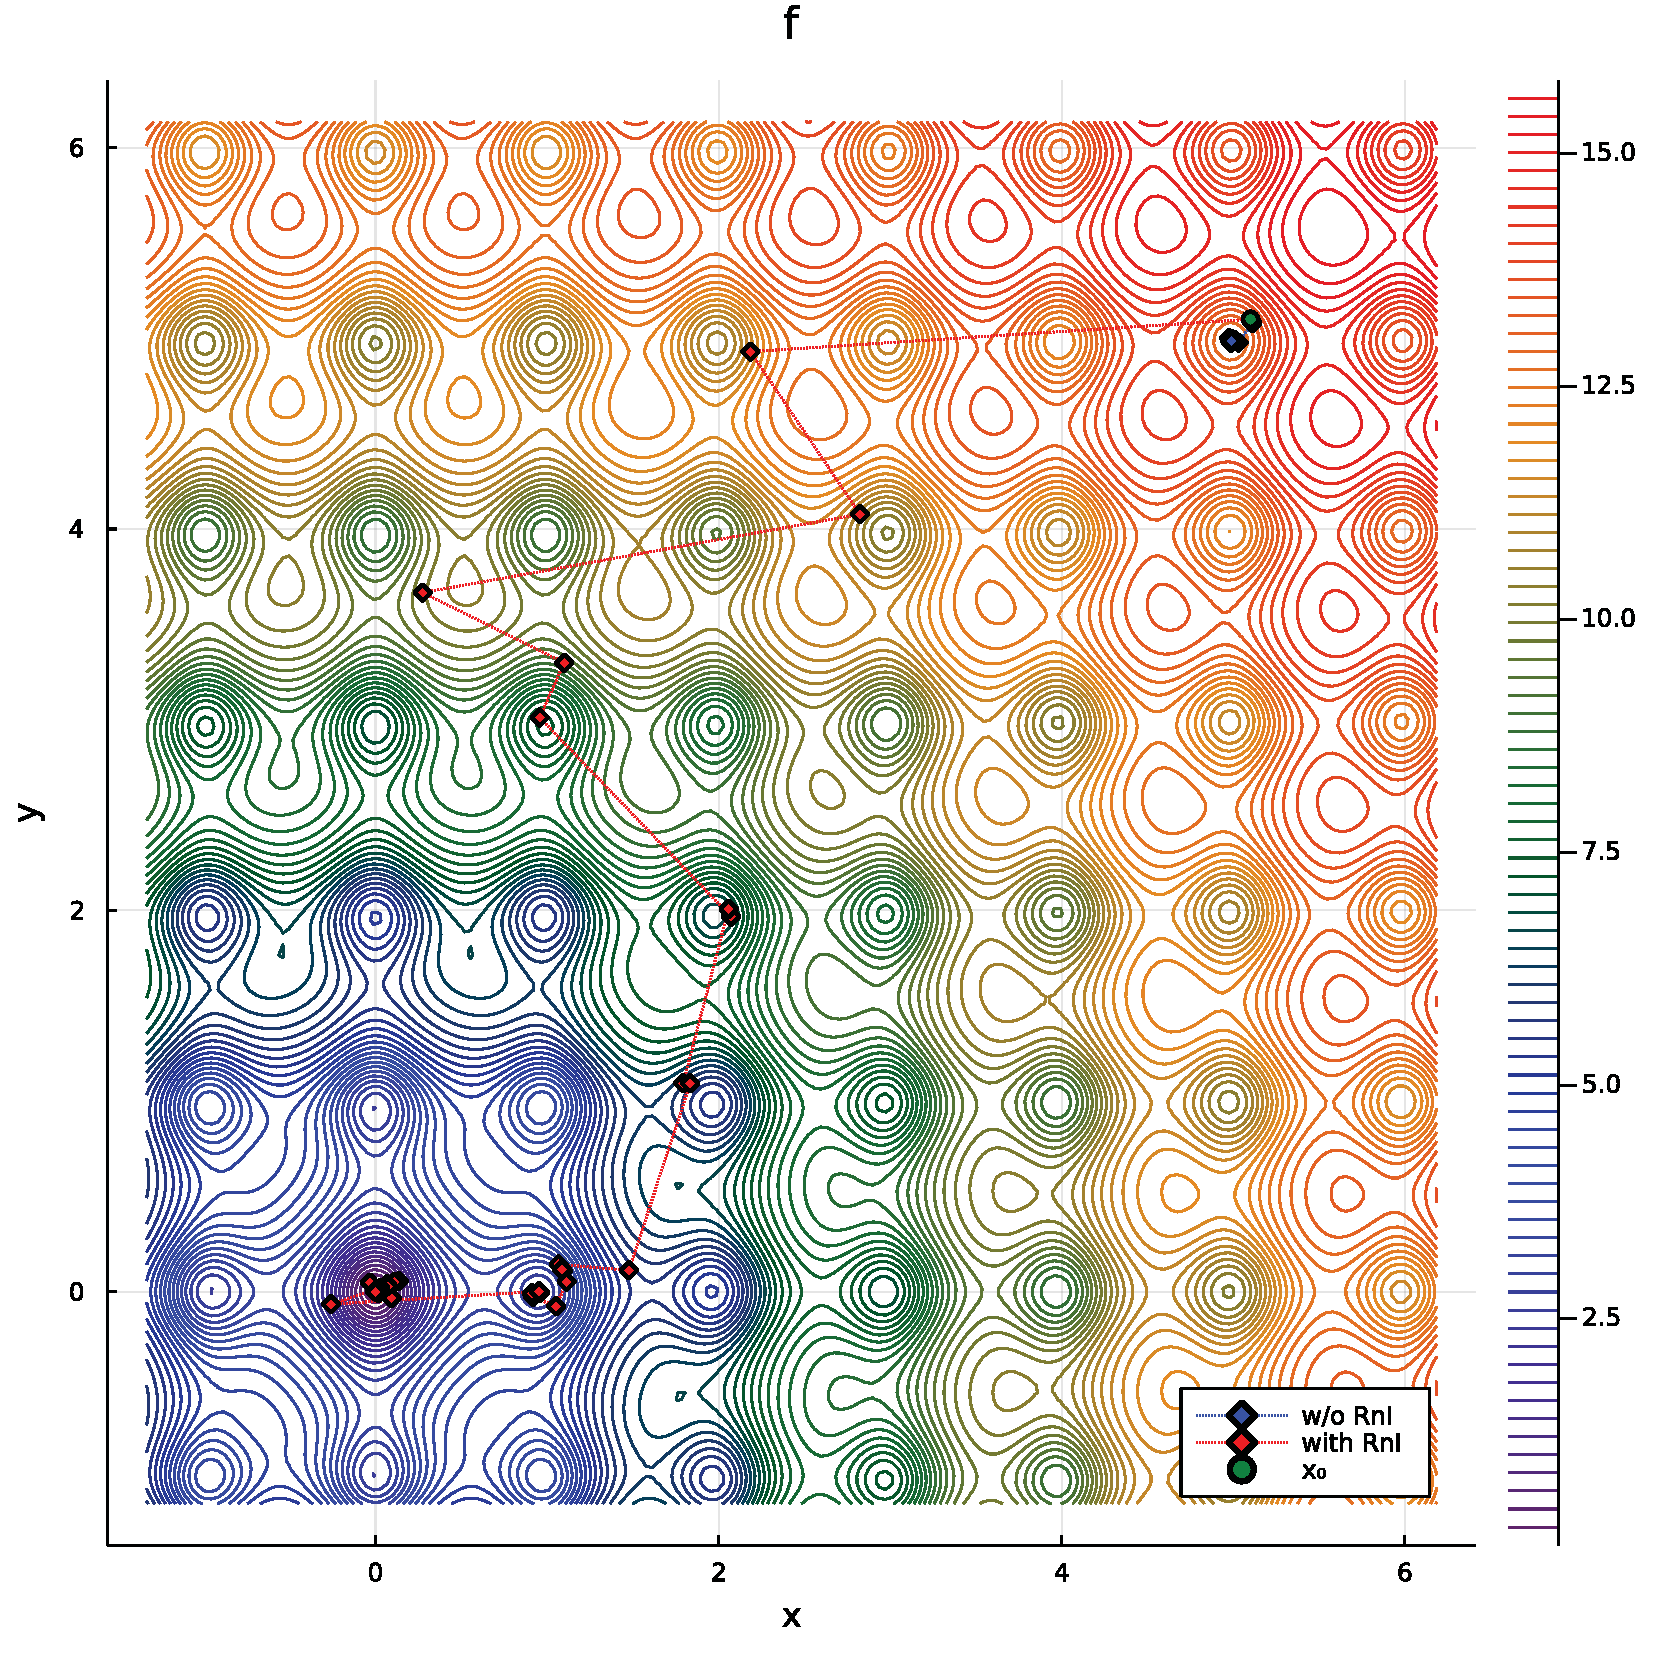
\includegraphics[width=0.48\linewidth]{fig/Ackley_sols.pdf}}
    \caption{Comparison of CARS and the Inspect-as-Running version of CARS for the Ackley function}
    \label{fig: Ackley}
\end{figure*}

The asymmetric Ackley function from \cite{chen2019run}
\begin{figure*}
    \centering
    \raisebox{-0.5\height}{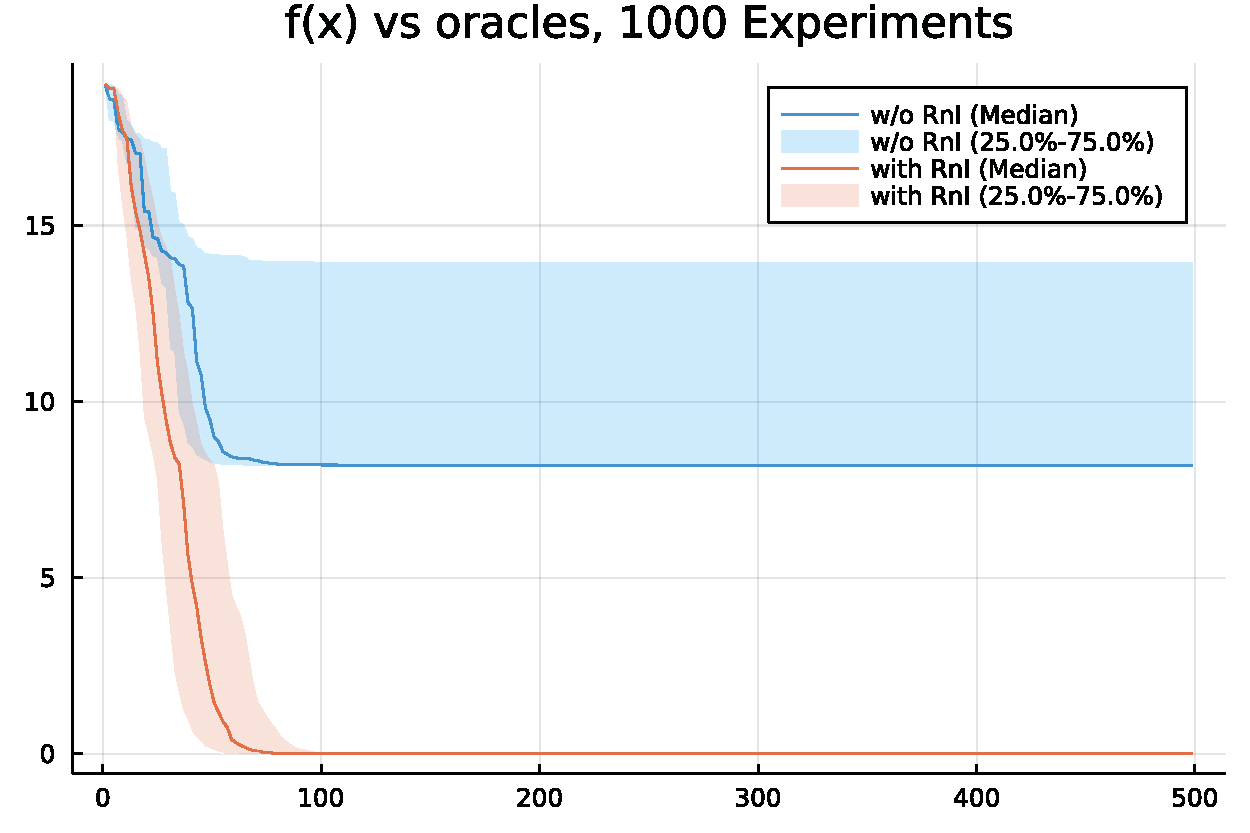
\includegraphics[width=0.48\linewidth]{fig/asym_Ackley.pdf}}
    \raisebox{-0.5\height}{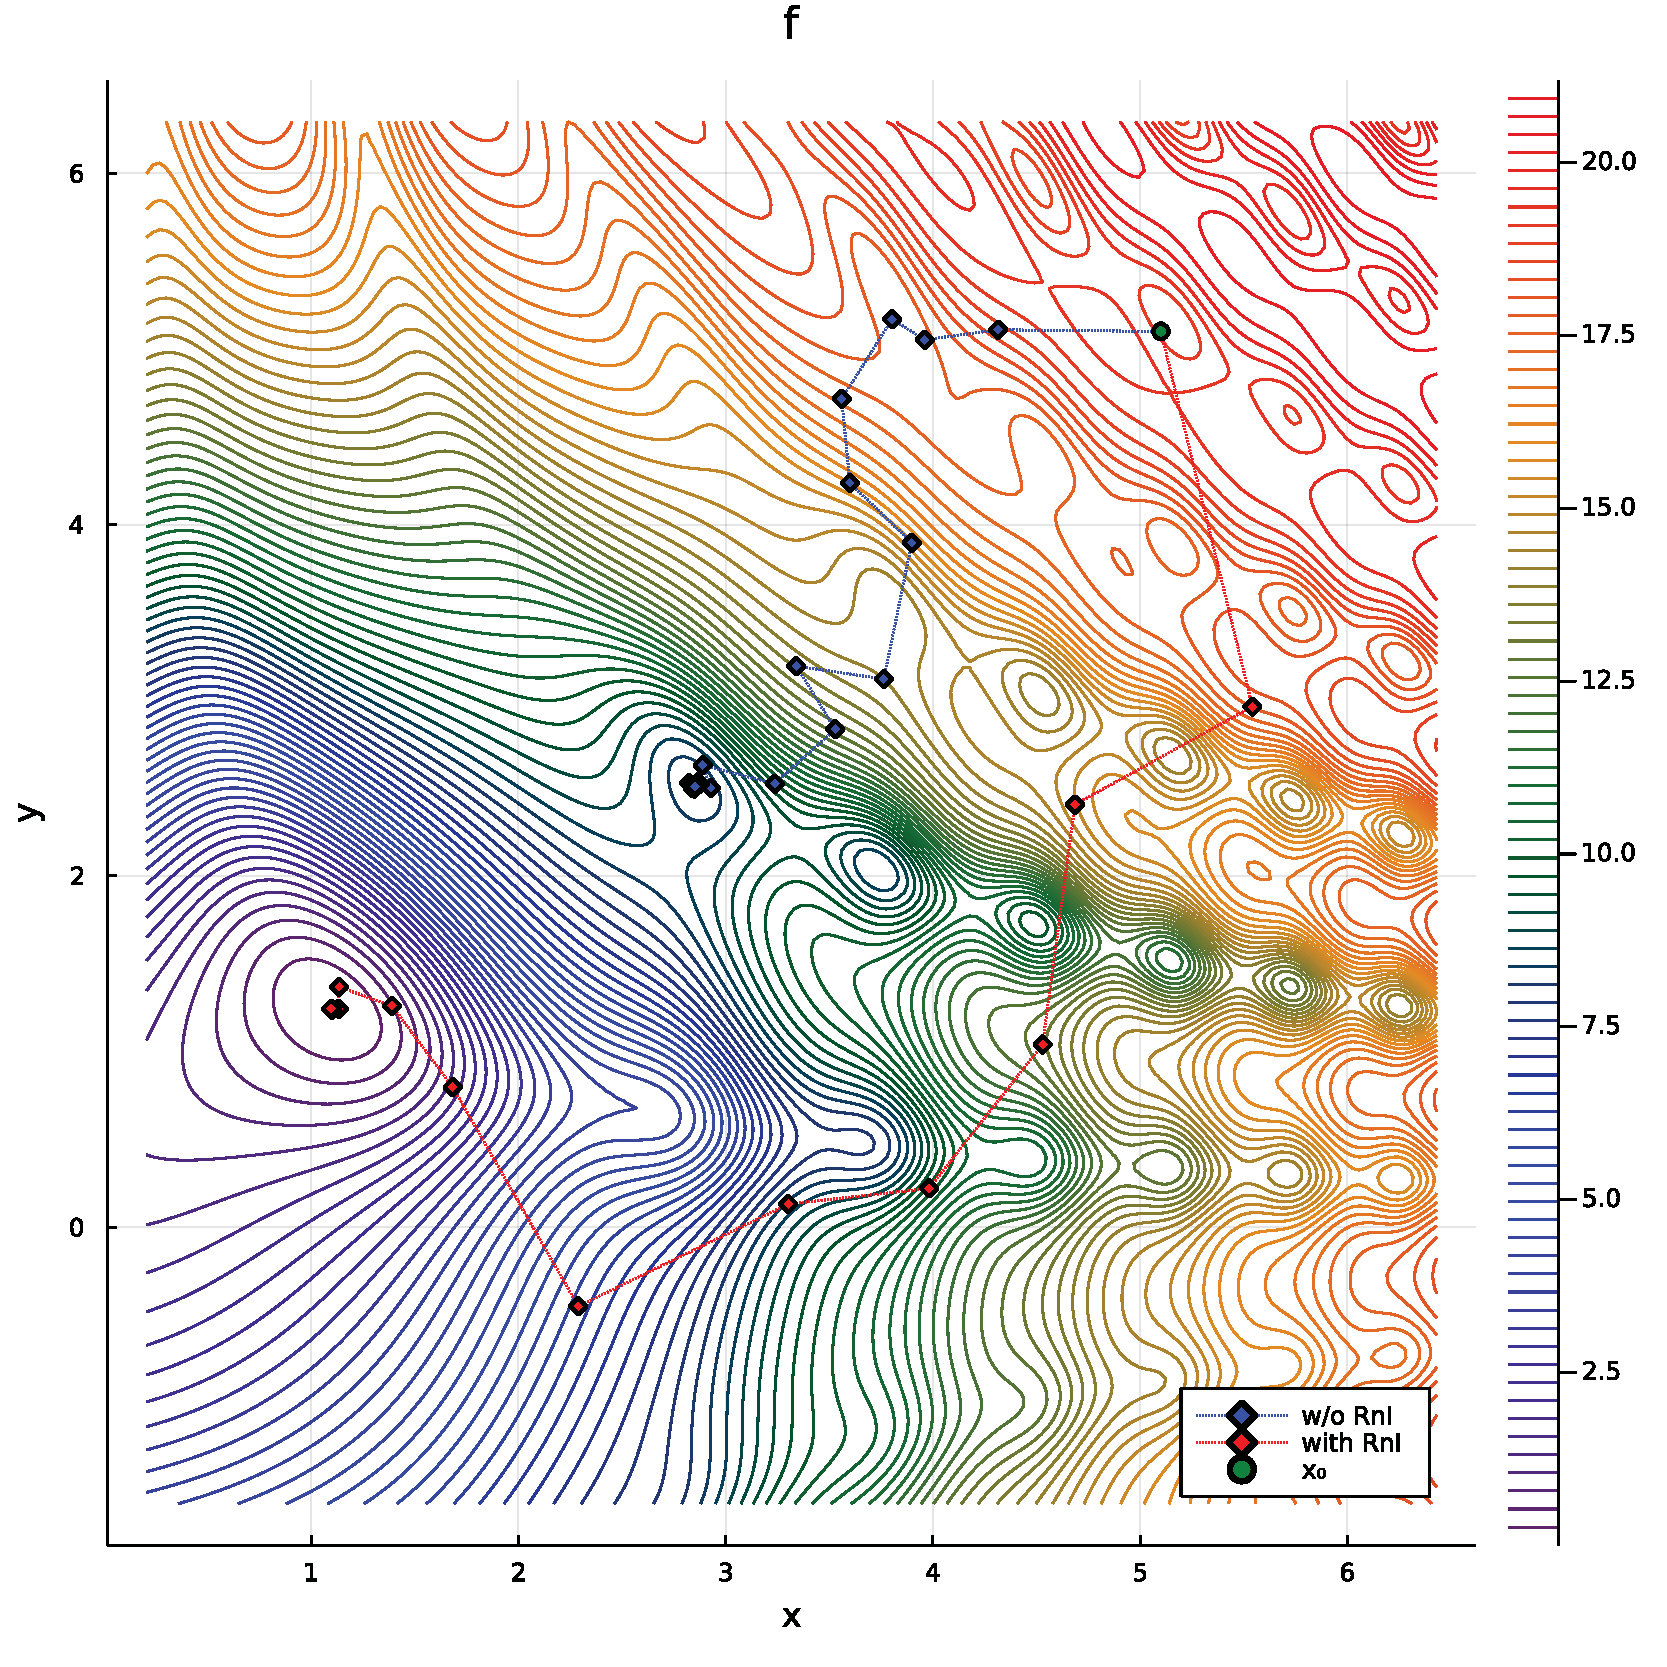
\includegraphics[width=0.48\linewidth]{fig/asym_Ackley_sols.pdf}}
    \caption{Comparison of CARS and the Inspect-as-Running version of CARS for the asymmetric Ackley function}
    \label{fig: Ackley asymmetric}
\end{figure*}

\subsection{K-means Clustering}
\subsubsection{Synthetic Gaussian data from \cite{yin2018stochastic}}

\begin{figure*}
    \centering
    \raisebox{-0.5\height}{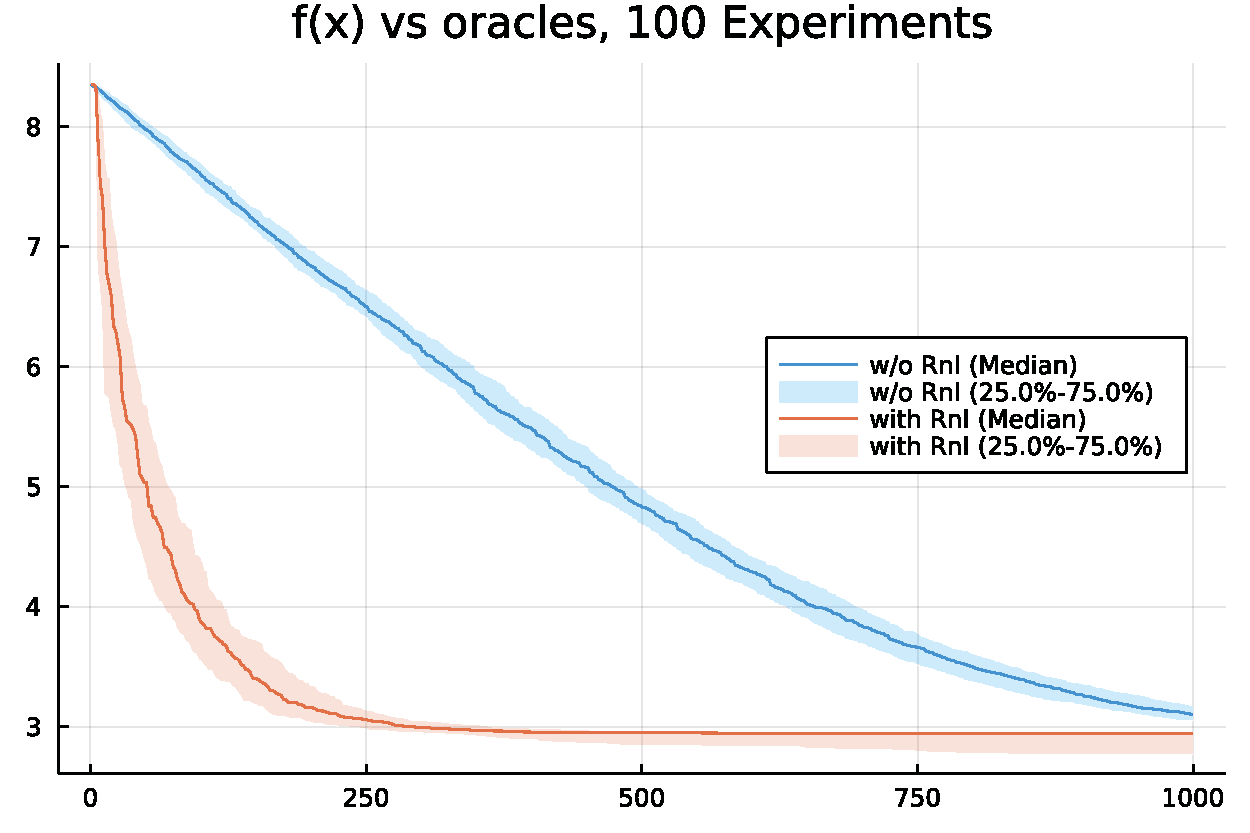
\includegraphics[width=0.48\linewidth]{fig/Kmeans_h0_0.136.pdf}}
    \raisebox{-0.5\height}{\includegraphics[width=0.48\linewidth]{fig/Kmeans_h0_0.136_2dplot.pdf}}
    \caption{Comparison of CARS and the Inspect-as-Running version of CARS for the K-means clustering problem of synthetic Gaussian data}
    \label{fig: K-means synthetic}
\end{figure*}

\subsubsection{Iris data}
\begin{figure*}
    \centering
    \raisebox{-0.5\height}{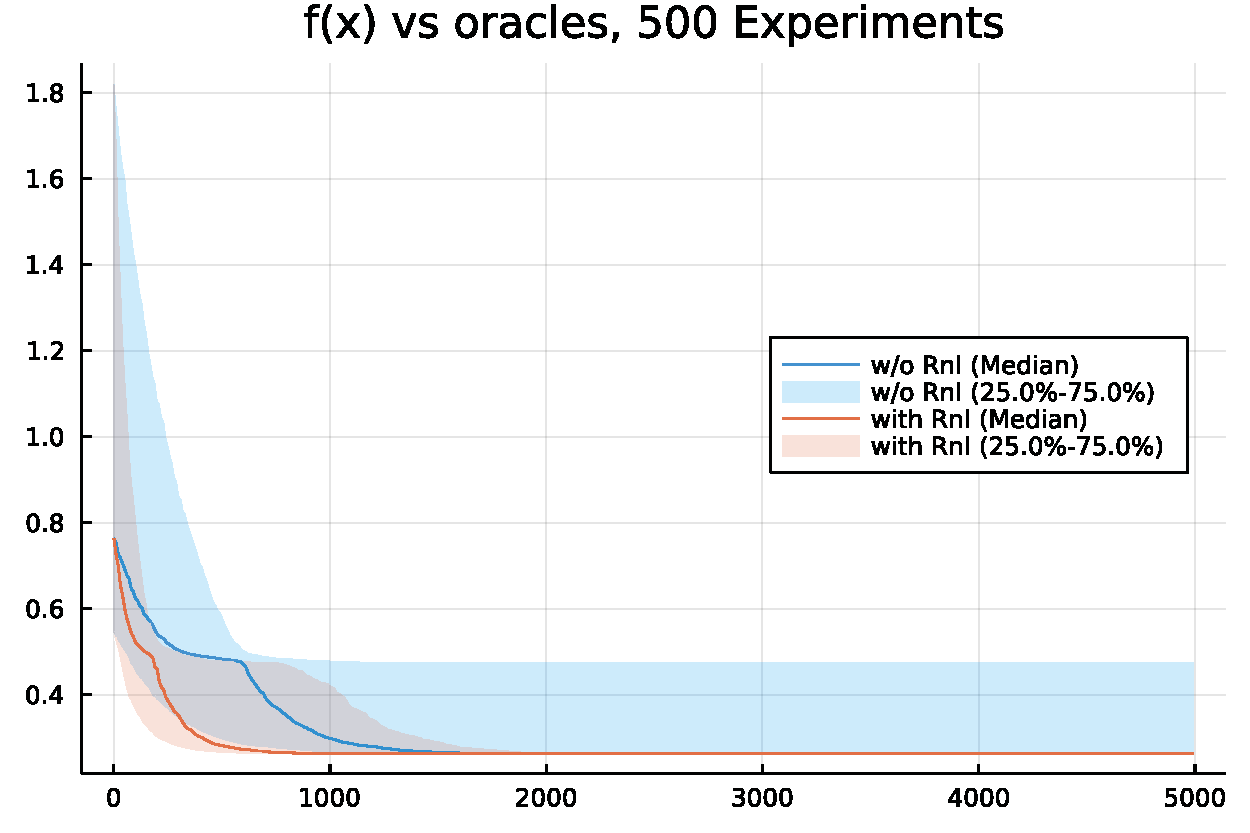
\includegraphics[width=0.48\linewidth]{fig/Iris_h0_1.36e-3_R3.pdf}}
    \raisebox{-0.5\height}{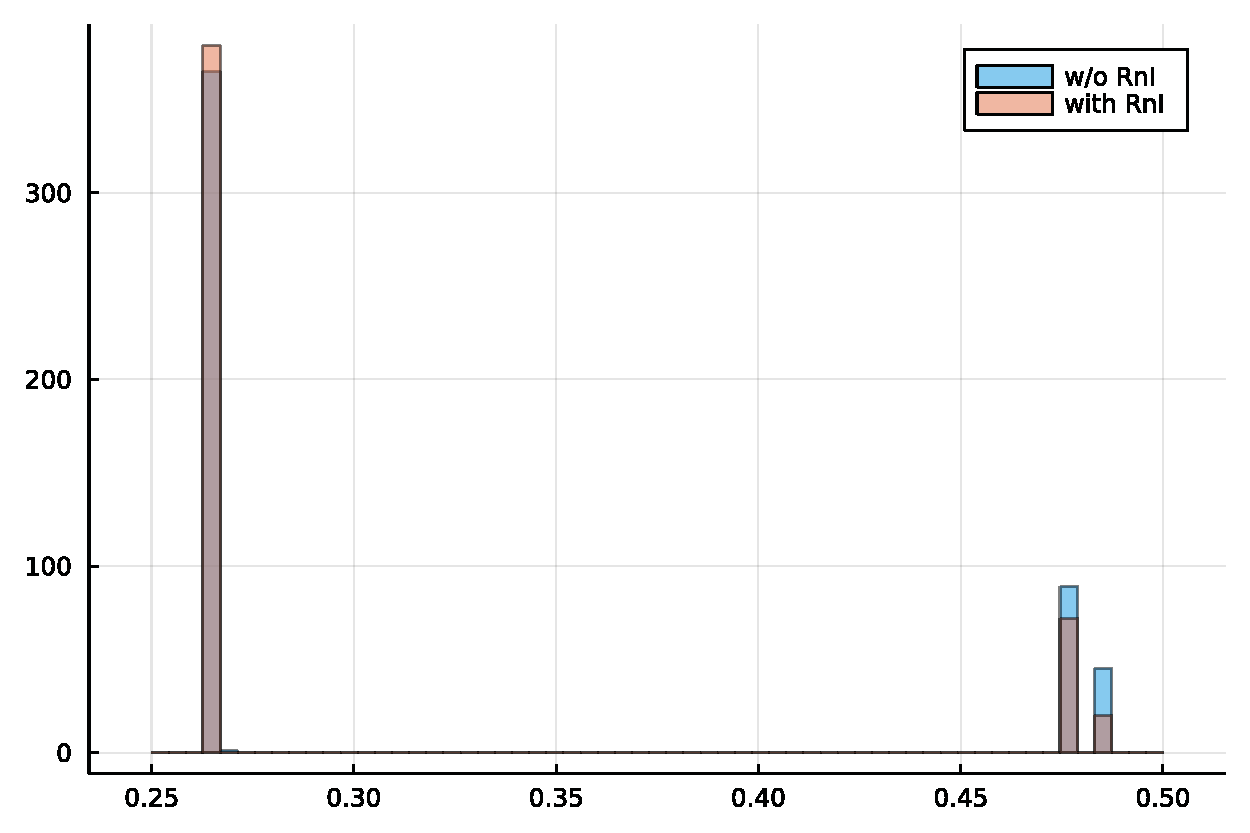
\includegraphics[width=0.48\linewidth]{fig/Iris_histogram.pdf}}
    \caption{Comparison of CARS and the Inspect-as-Running version of CARS for the K-means clustering of the Iris dataset}
    \label{fig: K-means Iris}
\end{figure*}
\subsection{Nonconvex robust linear regression}

\subsection{Hyperparameter tuning}
Hyperparameter tuning in training a convolutional neural network for classifying the MNIST dataset.
The hyperparameters were $L^2$ regularization parameter in the loss, the learning rate for the optimizer (AdaDelta), and the annealing rate for the scheduler (StepLR). To show the ability to escape the local minima more clearly, we started from a not an excellent point $x_0 = (0.5, 0.5, 0.5)$.

The objective function for the hyperparameter is set to be the mean of two samples, where each measures the misclassification rate of the trained model with the given set of hyperparameters.

\begin{figure*}
    \centering
    \raisebox{-0.5\height}{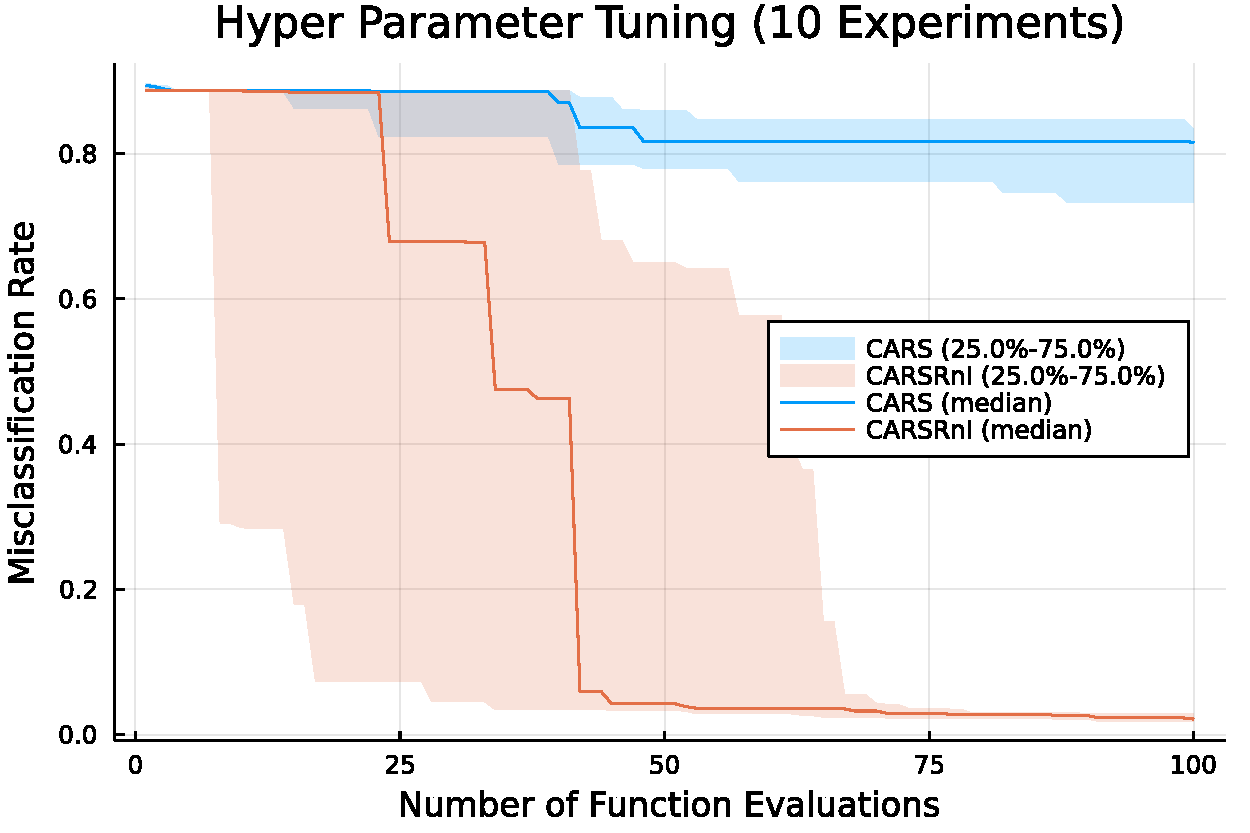
\includegraphics[width=0.48\linewidth]{fig/CARS_vs_CARSRnI_julia.pdf}}
    \raisebox{-0.5\height}{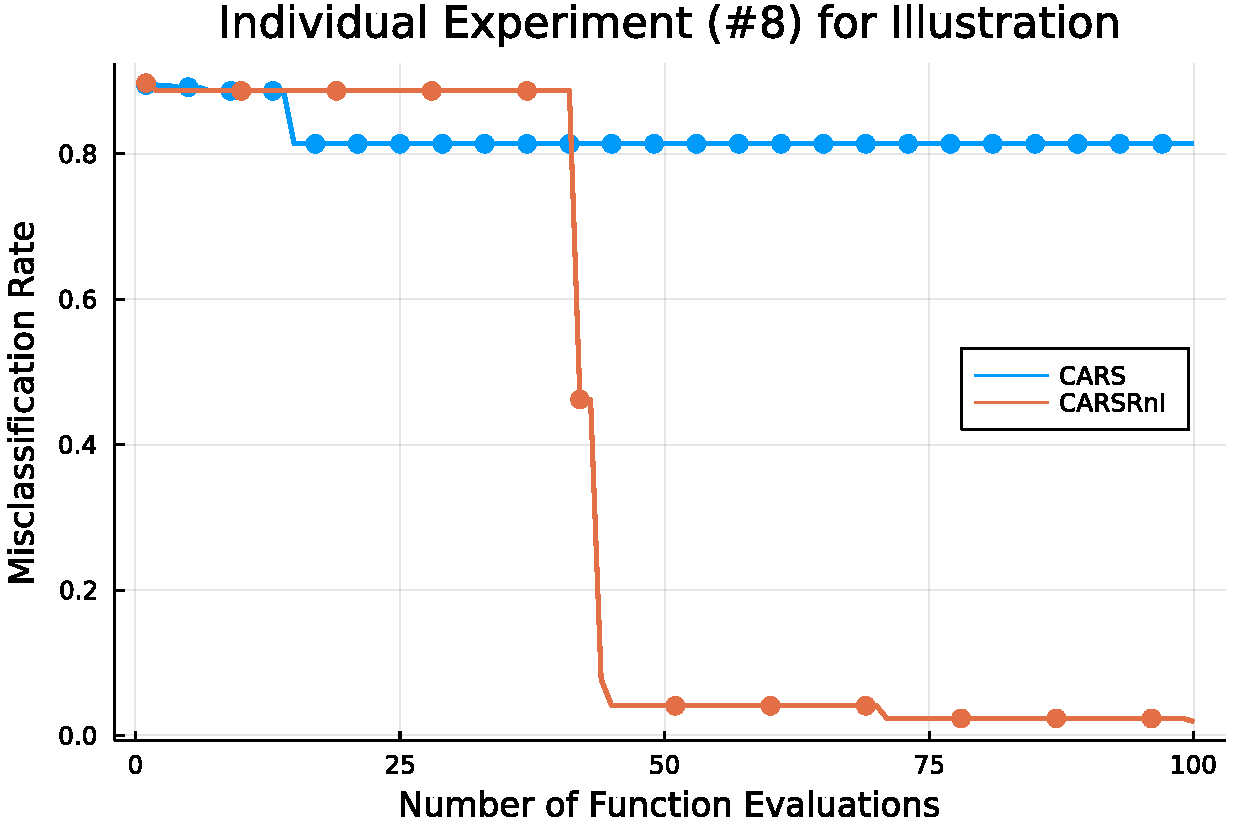
\includegraphics[width=0.48\linewidth]{fig/CARS_vs_CARSRnI_Individual_julia.pdf}}
    \caption{Comparison of CARS and the Inspect-as-Running version of CARS for hyperparameter tuning for training a convolutional neural network for MNIST dataset}
    \label{fig: HP Tuning - MNIST}
\end{figure*}



% \section{Introduction}
% We consider minimizing a function $f: \mathbb{R}^{d}\to \mathbb{R}$, with only access to function evaluations $f(x)$, and no access to gradients or directional derivatives. This setting is commonly referred to as derivative-free optimization (DFO). DFO has a rich history and has recently gained popularity in various areas such as reinforcement learning \cite{salimans2017evolution,mania2018simple,choromanski2020provably}, hyperparameter tuning \cite{bergstra2012random}, and adversarial attacks on neural network classifiers \cite{chen2017zoo,cai2020zeroth}. In all of these applications, evaluating $f(x)$ is either expensive, time-consuming, or inconvenient, and therefore, it is desirable for DFO algorithms to minimize the number of function evaluations required.

% \paragraph{Organization.}
% This paper is laid out as follows. In the rest of this section, we fix the notation and discuss prior art. In Section~\ref{sec:CARS}, we introduce the main algorithm, namely Curvature-Aware Random Search (CARS), along with its convergence analysis. 
% Section~\ref{section:CARS_CR} extends CARS with Cubic Regularization (CARS-CR) for general convex functions. In Section~\ref{sec: proofs of main results}, we provide mathematical proofs to support our technical claims. Section~\ref{sec:ExperimentalResults} contains extensive numerical experiments that empirically verify our technical claims. Section~\ref{sec:conclusion} concludes the paper.

% \subsection{Assumptions and Notation}
% \label{sec:Notation} 
% In developing and analyzing CARS, we assume that $f$ is a convex and twice continuously differentiable function. We use $g(x) = \nabla f(x)$ and $H(x) = \nabla^2 f(x)$ briefly in the theoretical analysis of Section~\ref{section:convergence of CARS}. For a fixed initial point $x_0$, we define the level-set $\mathcal{Q} = \{x\in\mathbb{R}^d : f(x)\leq f(x_0)\}$, $\|\cdot\|$ as the Euclidean norm, and $f_{\star} := \min_{x\in\mathbb{R}^{d}}f(x)$. We say $x_k$ is an $\varepsilon$-optimal solution if $f(x_k) - f_{\star} \leq \varepsilon$. We use $\mathcal{D}$ to denote a probability distribution on $\mathbb{R}^{d}$. For any measurable set $S \subseteq \mathbb{R}^{d}$ with finite measure, $\mathrm{Unif}(S)$ denotes the uniform distribution over $S$. The unit sphere is written as $\mathbb{S}^{d-1}:= \{u: \|u\| = 1\}\subseteq \mathbb{R}^{d}$, and $e_1,\cdots, e_d$ represent the canonical basis vectors in $\mathbb{R}^{d}$. For two matrices $A$ and $B$, we write $A\preceq B$ if $B-A$ is positive semi-definite.



% \subsection{Prior Art}
% \label{sec:PriorArt}

% For a comprehensive introduction to DFO we refer the reader to \cite{conn2009introduction} or the more recent survey article \cite{larson2019derivative}. As mentioned above, our interest is in ZO approaches to DFO \cite{liu2020primer}, as these have low per-iteration query complexity (with respect to the dimension of the problem) and have been successfully used in modern machine learning applications, such as adversarial attacks on neural networks \cite{chen2017zoo,liu2018zeroth, cheng2019sign, cai2020zeroth,cai2021zeroth} and reinforcement learning \cite{salimans2017evolution,choromanski2018structured,fazel2018global}. Of particular relevance to this work is ZO algorithms based on {\em line search}:


% \subsection{Main Contributions}
% We propose a simple and lightweight zeroth-order algorithm: CARS. To derive convergence rates for CARS we use a novel convergence analysis that hinges on the insight that CARS need only significantly decrease the objective function on a positive proportion of the iterates. Our results allow for a H\"{o}lder continuous Hessian---a weaker assumption than the Lipschitz continuity typically considered in such settings.  We also propose a cubic-regularized variant, CARS-CR. The analysis of CARS-CR extends that of the Stochastic Subspace Newton method \cite{pmlr-v119-hanzely20a} to the zeroth-order setting. The key ingredient is a careful handling of the errors introduced by replacing directional derivatives with their finite difference counterparts. Our theoretical results are corroborated by rigorous benchmarking on two datasets: Mor\'{e}-Garbow-Hillstrom \cite{more1981testing} and CUTEst \cite{gould2015cutest}, which reveal that CARS outperforms existing line-search based ZOO algorithms.  Our paper is accompanied by an open-source implementation of CARS (and CARS-CR), available online at \url{https://github.com/bumsu-kim/CARS}.


% \section{Curvature-Aware Random Search}\label{sec:CARS}
% Given $u_k$ sampled from $\mathcal{D}$, consider the one-dimensional Taylor expansion:

% \section{CARS with Cubic Regularization for General Convex Functions}
% \label{section:CARS_CR}
% Here, we adopt cubic regularization \cite{nesterov2006cubic, pmlr-v119-hanzely20a}, a technique to achieve global convergence of a second-order method for convex functions, in CARS and prove convergence.


% \section{Proofs}
% \label{sec: proofs of main results}

% Here we collect the proofs of the results of Sections \ref{section:convergence of CARS} and \ref{section:CARS_CR}, and state and prove some auxiliary lemmas needed in the proofs of the main results. We begin with a lemma quantifying the expected descent given access to exact derivatives.


% \section{Experimental Results}
% \label{sec:ExperimentalResults}
% For a detailed description of all experimental settings and hyperparameters, see Appendix~\ref{appendix: Experiments}. The code for all the experiments can be found online at \url{https://github.com/bumsu-kim/CARS}.


% \section{Conclusion Remarks} \label{sec:conclusion}
% We proposed two query-efficient and lightweight DFO algorithms: CARS and CARS-CR. Our analysis establishes their convergence on strongly convex functions and convex functions. Specifically, we develop a novel and rigorous analysis on the finite difference errors and the probability of significant descents of the objective function. CARS can incorporate various distributions, making it highly adaptable to a range of problem-specific distributions. We demonstrate the efficacy of CARS and CARS-CR through benchmark tests, where it outperforms existing methods in  minimizing non-convex functions as well. 

% \section*{Declarations}
% \begin{itemize}
% \item Funding: The work of HanQin Cai is partially supported by NSF DMS 2304489.
% \item Conflict of interest: The authors have no conflicts of interest to declare that are relevant to the content of this article.
% \item Code availability: The software code of this paper can be accessed through https://github.com/bumsu-kim/CARS
% \end{itemize}

\bibliography{realbib}

% \appendix
% \section{More on Numerical Experiments}\label{appendix: Experiments}
% In this section, we list the hyperparameters we used for each experiment. The code for all experiments can be found in \url{https://github.com/bumsu-kim/CARS}. We ran experiments on two machines to distribute the load. A laptop equipped with Intel i5-9400F and Nvidia RTX 2060 and a workstation equipped with i9-9940X and two Nvidia RTX 2080 are used.


\end{document}
